\ifx\wholebook\relax \else
% ------------------------

\documentclass[b5paper]{article}

\usepackage[en]{../../prelude}

\setcounter{page}{1}

\begin{document}

\title{Preface}

\author{Xinyu LIU
\thanks{{\bfseries Xinyu LIU} \newline
  Email: liuxinyu95@gmail.com \newline}
  }

\maketitle
\fi

\markboth{Preface}{Elementary Algorithms}

\chapter*{Preface}
\phantomsection  % so hyperref creates bookmarks
\addcontentsline{toc}{chapter}{Preface}

Programmers learn elementary algorithms at school. Except for programming contest or code interview, they seldom develop algorithms at work. Most time, the needed algorithms or data structures are provided in libraries. We needn't bother to `re-invent the wheel'. When talking about algorithms in AI and machine learning, people actually mean scientific modeling. Elementary algorithms are fundamental things, Let's start with two puzzles.

\section*{The smallest free number}
\label{min-free} \index{minimum free number}

Richard Bird gives a problem to find the minimum number that not appears in a list (Chapter 1, \cite{fp-pearls}). People use number to index entities. A number is either occupied or free. When acquire, we always want to allocate the smallest available one. Suppose numbers are non-negative integers and those being used are recorded in a list, for example:

\begin{Verbatim}[fontsize=\footnotesize]
[18, 4, 8, 9, 16, 1, 14, 7, 19, 3, 0, 5, 2, 11, 6]
\end{Verbatim}

How can we find the smallest free number, 10, from this list? It seems quite easy with exhaustive search:

\begin{algorithmic}[1]
\Function{Min-Free}{$A$}
  \State $x \gets 0$
  \Loop
    \If{$x \notin A$}
      \State \Return $x$
    \Else
      \State $x \gets x + 1$
    \EndIf
  \EndLoop
\EndFunction
\end{algorithmic}

Where the $\notin$ is realized as below.

\begin{algorithmic}[1]
\Function{`$\notin$'}{$x, X$}
  \For{$i \gets 1 $ to $|X|$}
    \If{$x = X[i]$}
      \State \Return False
    \EndIf
  \EndFor
  \State \Return True
\EndFunction
\end{algorithmic}

Where $|X| = n$ is the length of $X$. Some environments have built-in implementation to test existence of an element. However, this solution performs poor with millions of numbers. The time spent is quadratic to $n$. In a computer with 2 cores of 2.10 GHz CPU, and 2G RAM, the C implementation takes 5.4s to find the answer among 100K numbers, and exceeds 8 minutes to handle 1 million numbers.

\subsection*{Improvement}
For $n$ numbers $x_1, x_2, ..., x_n$, if there is a free number, some $x_i$ must be out of the range $[0, n)$\footnote{Range $[a, b)$ starts from $a$ to $b$, but excludes $b$.}; otherwise the list is exactly some permutation of $0, 1, ..., n - 1$ hence $n$ is the minimum free number.

\be
\textit{minfree}(x_1, x_2, ..., x_n) \leq n
\label{eq:min-free}
\ee

We use an array $F$ of $n + 1$ flags to mark whether a number is free in $[0, n]$.

\begin{algorithmic}[1]
\Function{Min-Free}{$A$}
  \State $F \gets $[False, False, ..., False] \Comment{$n+1$}
  \For{$x$ in $A$}
    \If{$x < n$}
      \State $F[x] \gets$ True
    \EndIf
  \EndFor
  \For{$i \gets 0$ to $n$}
    \If{$F[i] =$ False}
      \State \Return $i$
    \EndIf
  \EndFor
\EndFunction
\end{algorithmic}

Initialize $F$ with all False values. For every number $x$ in $A$, mark the flag $F[x]$ true if $x < n$. Finally, scan $F$ to find the first false flag. This program takes time proportion to $n$. It uses $n + 1$ flags to cover the special case that $sort(A) = [0, 1, 2, ..., n-1]$. To avoid repeated allocate then release the flags, we can pre-allocate a sufficient big buffer for reusing, and change to bit-wise flags instead of array. The C implementation handles 1 million numbers in 0.023s in the same computer.

%% \begin{lstlisting}[language=C]
%% #define N 1000000
%% #define WORD_LENGTH (sizeof(int) * 8)

%% void setbit(unsigned int* bits, unsigned int i) {
%%     bits[i / WORD_LENGTH] |= 1 << (i % WORD_LENGTH);
%% }

%% int testbit(unsigned int* bits, unsigned int i) {
%%     return bits[i / WORD_LENGTH] & (1 << (i % WORD_LENGTH));
%% }

%% unsigned int bits[N / WORD_LENGTH + 1];

%% int minfree(int* xs, int n) {
%%   int i, len = N/WORD_LENGTH + 1;
%%   for (i = 0; i < len; ++i) {
%%       bits[i]=0;
%%   }
%%   for (i=0; i < n; ++i) {
%%       if(xs[i] < n) {
%%           setbit(bits, xs[i]);
%%       }
%%   }
%%   for (i=0; i <= n; ++i) {
%%       if (!testbit(bits, i)) {
%%           return i;
%%       }
%%   }
%% }
%% \end{lstlisting}

\subsection*{Divide and Conquer}
The divide and conquer method breaks the problem into smaller ones, then solve them and consolidate the result. Collect $x_i \leq \lfloor n/2 \rfloor$ in sub-list $A'$ and the rest in another $A''$. According to \cref{eq:min-free}, if the length of $|A'| = \lfloor n/2 \rfloor$, it means $A'$ is `full'. The minimum free number must be in $A''$, otherwise in $A'$. Both cases lead to a smaller problem. When search in $A''$, we start from $\lfloor n/2 \rfloor + 1$, but not from $0$. We define the algorithm as $search(A, l, u)$, where $l$ and $u$ are the lower and upper bounds. We start from $minfree(A) = search(A, l = 0, u = |A|-1)$:

\[
\begin{array}{rcl}
search(\nil, l, u) & = & l \\
search(A, l, u) & = & \begin{cases}
       |A'| = m - l + 1 : & search(A'', m+1, u) \\
       otherwise : & search(A',  l, m) \\
\end{cases}
\end{array}
\]

where:

\[
\begin{cases}
m = \lfloor \dfrac{l + u}{2} \rfloor \\
A' = [x \leq m, x \in A], A'' = [x > m, x \in A] \\
\end{cases}
\]

This algorithm needn't additional space\footnote{The recursion takes $O(\lg n)$ stack spaces, but it can be eliminated through tail recursion optimization}. Each recursive call performs $O(|A|)$ comparisons to partition $A'$ and $A''$, hence halves the problem as $T(n) = T(n/2) + O(n)$. We can reduce it to $O(n)$ according to the master theorem\footnote{Alternatively, the first call takes $O(n)$ time to partition $A'$ and $A''$, the second call takes $O(n/2)$ time, the third call takes $O(n/4)$ time ... The total time is $O(n + n/2 + n/4 + ...) = O(2n) = O(n)$.}. Below example program in Haskell implements this algorithm.

\lstset{frame = single}
\begin{Haskell}
minFree xs = bsearch xs 0 (length xs - 1)

bsearch xs l u | xs == [] = l
               | length as == m - l + 1 = bsearch bs (m + 1) u
               | otherwise = bsearch as l m
    where
      m = (l + u) `div` 2
      as = [x | x <- xs, x <= m]
      bs = [x | x <- xs, x > m]
\end{Haskell}

There are $O(\lg n)$ recursive calls. We can eliminate the recursion with loops:

\begin{algorithmic}[1]
\Function{Min-Free}{$A$}
  \State $l \gets 0, u \gets |A|$
  \While{$u - l > 0$}
    \State $m \gets \lfloor \dfrac{u + l}{2} \rfloor$
    \State $left \gets l$
    \For{$right \gets l$ to $u - 1$}
      \If{$A[right] \leq m$}
        \State Exchange $A[left] \leftrightarrow A[right]$
        \State $left \gets left + 1$
      \EndIf
    \EndFor
    \If{$left < m + 1$}
      \State $u \gets left$
    \Else
      \State $l \gets left$
    \EndIf
  \EndWhile
\EndFunction
\end{algorithmic}

As shown in \cref{fig:divide}, this program re-arranges the array such that all elements before $left$ are less than or equal to $m$; while those between $left$ and $right$ are greater than $m$.

\begin{figure}[htbp]
  \centering
  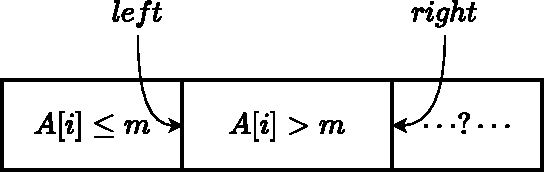
\includegraphics[scale=0.7]{img/partition-by}
  \caption{All $A[i] \leq m$ where $0 \leq i < left$; while $A[i] > m$ where $left \leq i < right$. The rest are yet to be scanned.}
  \label{fig:divide}
\end{figure}

\section*{Regular number}

The second problem is to find the 1,500-th number, which only contains factor 2, 3 or 5. Such numbers are called the regular numbers\footnote{Also known as 5-smooth numbers in number theory, and Hamming numbers named after Richard Hamming.}. 2, 3, and 5 are definitely regular numbers. $60 = 2^23^15^1$ is the 25-th regular number. $21 = 2^03^17^1$ is not because it has a factor of 7. Define $1=2^03^05^0$ as the 0-th regular number. The first 10 are:

1, 2, 3, 4, 5, 6, 8, 9, 10, 12, ...

\subsection*{The brute-force solution}
We can check numbers one by one from 1, extract all factors of 2, 3 and 5 to see if the remaining is 1:

\begin{algorithmic}[1]
\Function{Regular-Number}{$n$}
  \State $x \gets 1$
  \While{$n > 0$}
    \State $x \gets x + 1$
    \If{\Call{Valid?}{$x$}}
      \State $n \gets n - 1$
    \EndIf
  \EndWhile
  \State \Return $x$
\EndFunction
\Statex
\Function{Valid?}{$x$}
  \While{$x \bmod 2 = 0$}
    \State $x \gets x / 2$
  \EndWhile
  \While{$x \bmod 3 = 0$}
    \State $x \gets x / 3$
  \EndWhile
  \While{$x \bmod 5 = 0$}
    \State $x \gets x / 5$
  \EndWhile
  \State \Return $x = 1$ ?
\EndFunction
\end{algorithmic}

This `brute-force' algorithm performs poor when $n$ increases. The C implementation takes 40.39s in above computer to find the 1500-th number (860934420).

\subsection*{Improvement}
Modular and divide are expensive operations\cite{Bentley}. Instead of checking every number, we can generate regular numbers from 1 in ascending order. We use a queue, which allows to add number to one end (enqueue), and remove from the other end (dequeue). The number enqueued first will be dequeued first (First In First Out). Initialize the queue with 1, the 0th regular number. We repeatedly dequeue a number, multiply it by 2, 3, 5 to generate 3 new numbers; then add them to the queue in ascending order. We drop the number if it is already in the queue, as shown in \cref{fig:queues}.

\begin{figure}[htbp]
  \centering
  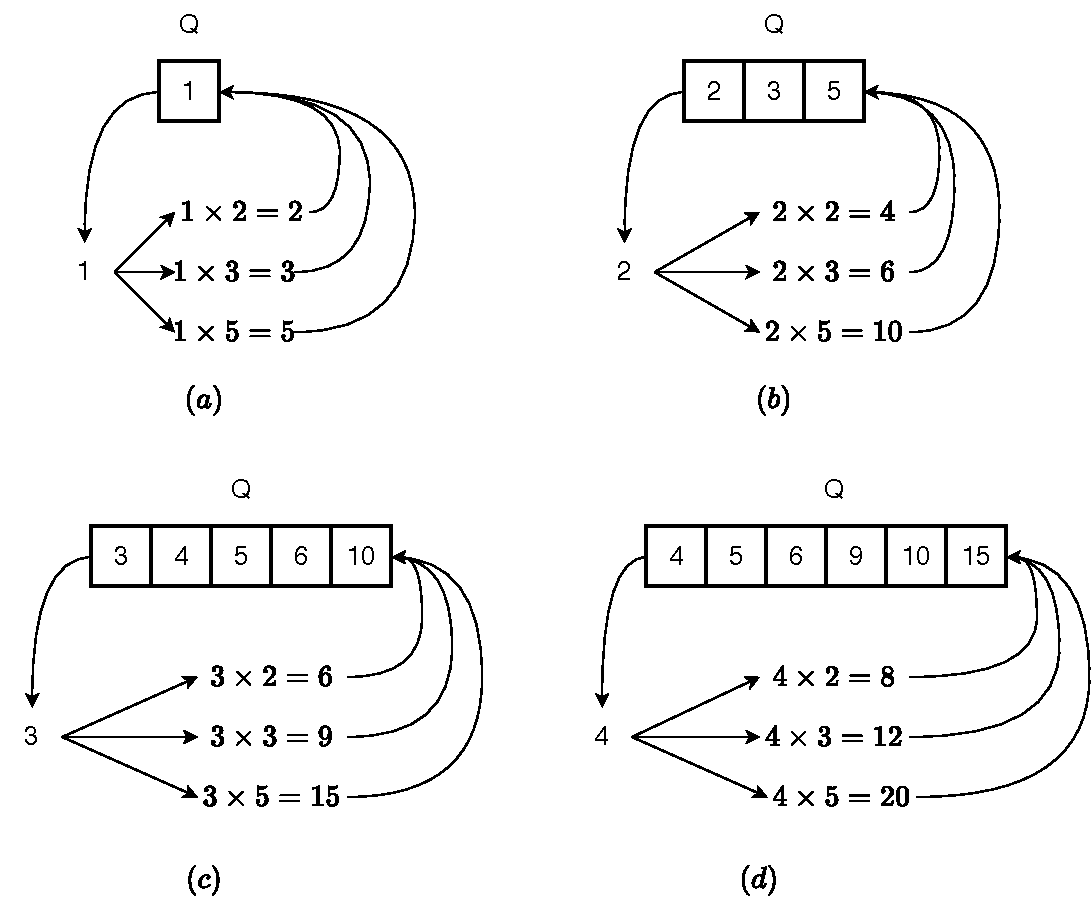
\includegraphics[scale=0.5]{img/regular-num-1q}
  \caption{First 4 steps.}
  \label{fig:queues}
\end{figure}

\begin{algorithmic}[1]
\Function{Regular-Number}{$n$}
  \State $Q \gets [1]$
  \While{$n > 0$}
    \State $x \gets$ \Call{Dequeue}{$Q$}
    \State \Call{Unique-Enqueue}{$Q, 2x$}
    \State \Call{Unique-Enqueue}{$Q, 3x$}
    \State \Call{Unique-Enqueue}{$Q, 5x$}
    \State $n \gets n-1$
  \EndWhile
  \State \Return $x$
\EndFunction
\Statex
\Function{Unique-Enqueue}{$Q, x$}
  \State $i \gets 0, m \gets |Q|$
  \While{$i < m$ and $Q[i] < x$}
    \State $i \gets i + 1$
  \EndWhile
  \If{$i \geq m$ or $x \neq Q[i]$}
    \State \Call{Insert}{$Q, i, x$}
  \EndIf
\EndFunction
\end{algorithmic}

The \textproc{Unique-Enqueue} function takes $O(m)$ time to uniquely insert a number in ascending order, where $m = |Q|$ is the length of the queue. It increases proportion to $n$ (Each time, we dequeue an element, and enqueue at most 3. The increasing ratio $\leq$ 2), the total time is $O(1 + 2 + 3 + ... + n) = O(n^2)$. \Cref{fig:big-O-1q} shows the queue access times against $n$. The quadratic curve reflects the $O(n^2)$ performance.

\begin{figure}[htbp]
  \centering
  \includegraphics[scale=0.5]{img/big-O-1q}
  \caption{Queue access count - $n$.}
  \label{fig:big-O-1q}
\end{figure}

The corresponding C implementation takes 0.016s to output 860934420, about 2500 times faster than the brute-force solution. Let $xs = [x_1, x_2, x_3, ...]$ be the infinite list of all regular numbers. Multiply every number by 2, the result is again infinite many regular numbers: $[2x_1, 2x_2, 2x_3, ...]$, so as multiply by 3 and 5. If we merge the three infinite lists together, filter out the duplicated numbers, and prepend 1 as the first, we get $xs$ again:

\be
  xs = 1 : [2x | x \gets xs] \cup [3x | x \gets xs] \cup [5x | x \gets xs]
\ee

Where $x \cons xs$ links $x$ before list $xs$. It is called `cons' in Lisp. 1 is linked as the head (the 0th regular number). $\cup$ merges two lists:

\[
(a \cons as) \cup (b \cons bs) = \begin{cases}
  a < b: & a : as \cup (b \cons bs) \\
  a = b: & a : as \cup bs \\
  a > b: & b : (a \cons as) \cup bs \\
\end{cases}
\]

Below is the example program in Haskell:

\begin{Haskell}
xs = 1 : [2*x | x <- xs] `merge` [3*x | x <- xs] `merge` [5*x | x <- xs]

merge (a:as) (b:bs) | a < b = a : merge as (b:bs)
                    | a == b = a : merge as bs
                    | otherwise = b : merge (a:as) bs
\end{Haskell}

This example program in Haskell gives the 1500th number 860934420 by \texttt{xs !! 1500} in 0.03s in the same computer.

\subsection*{Queues}
The above solution needs filter out duplicated numbers, scan the queue to maintain the ascending order. We category all regular numbers into 3 disjoint buckets: $Q_2 = \{2^i | i > 0\}$, $Q_{23} = \{ 2^i3^j | i \geq 0, j > 0 \}$, and $Q_{235} = \{ 2^i3^j5^k | i,j \geq 0, k > 0\}$. Constraint $j \neq 0$ in $Q_{23}$, and $k \neq 0$ in $Q_{235}$ such there is no overlap. Realize the buckets as 3 queues starting from $Q_2 = \{ 2 \}$, $Q_{23} = \{ 3\}$, and $Q_{235} = \{ 5 \}$. Each time extract the smallest $x$ from the queues, then do the following:

\begin{itemize}
\item If $x$ comes from $Q_2$, enqueue $2x$ to $Q_2$, $3x$ to $Q_{23}$, and $5x$ to $Q_{235}$;
\item If $x$ comes from $Q_{23}$, enqueue $3x$ to $Q_{23}$, and $5x$ to $Q_{235}$. We do not add $2x$ to $Q_2$, because $Q_2$ does not hold any numbers divisible by 3.
\item If $x$ comes from $Q_{235}$, enqueue $5x$ to $Q_{235}$. We do not add $2x$ to $Q_2$, or $3x$ to $Q_{23}$ because they don't hold numbers divisible by 5.
\end{itemize}

We reach to the answer after dequeue $n$ numbers. \Cref{fig:q235} gives the first 4 steps.

\begin{figure}[htbp]
  \centering
  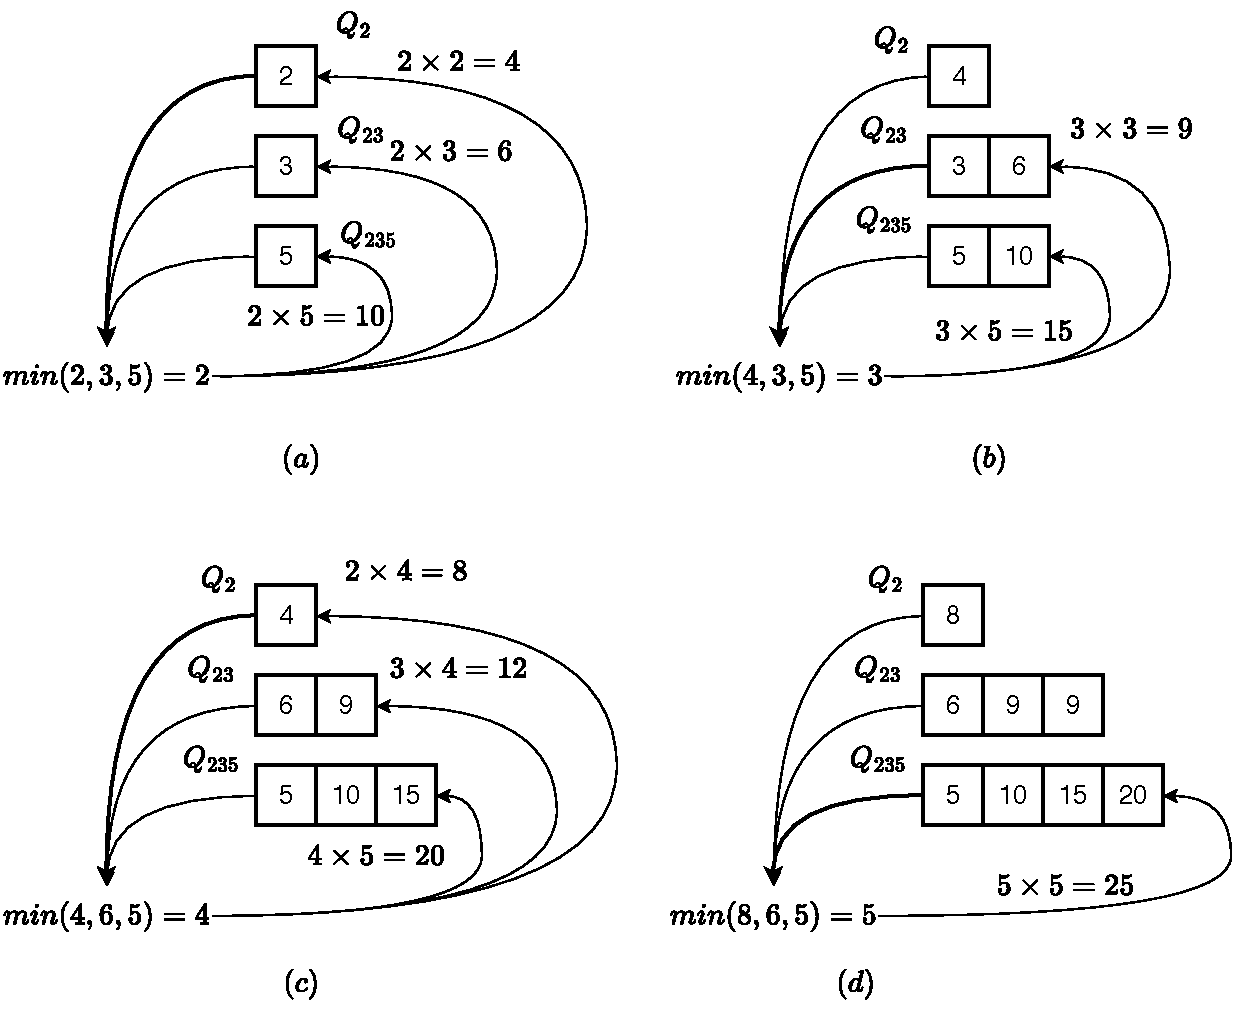
\includegraphics[scale=0.5]{img/q235}
  \caption{First 4 steps with $Q_2$, $Q_{23}$, and $Q_{235}$.}
  \label{fig:q235}
\end{figure}

\begin{algorithmic}[1]
\Function{Regular-Number}{$n$}
  \State $x \gets 1$
  \State $Q_2 \gets \{ 2 \}$, $Q_{23} \gets \{ 3 \}$, $Q_{235} \gets \{ 5 \}$
  \While{$n > 0$}
    \State $x \gets min$(\Call{Head}{$Q_2$}, \Call{Head}{$Q_{23}$}, \Call{Head}{$Q_{235}$})
    \If{$x =$ \Call{Head}{$Q_2$}}
      \State \Call{Dequeue}{$Q_2$}
      \State \Call{Enqueue}{$Q_2, 2x$}
      \State \Call{Enqueue}{$Q_{23}, 3x$}
      \State \Call{Enqueue}{$Q_{235}, 5x$}
    \ElsIf{$x=$ \Call{Head}{$Q_{23}$}}
      \State \Call{Dequeue}{$Q_{23}$}
      \State \Call{Enqueue}{$Q_{23}, 3x$}
      \State \Call{Enqueue}{$Q_{235}, 5x$}
    \Else
      \State \Call{Dequeue}{$Q_{235}$}
      \State \Call{Enqueue}{$Q_{235}, 5x$}
    \EndIf
    \State $n \gets n - 1$
  \EndWhile
  \State \Return $x$
\EndFunction
\end{algorithmic}

This algorithm loops $n$ times. Each time extracts the minimum number in constant time. Then adds at most 3 numbers to the queues in constant time. The overall performance is $O(n)$.

\section*{Summary}
Both brute-force solutions can't scale up. This book is {\em not} about coding contest or code interview, but aims to provide both purely functional algorithms and their counterpart imperative implementations. We referenced many results from Okasaki's work\cite{okasaki-book} and classic text books\cite{CLRS}. We avoid relying on a specific programming language, because the reader may or may not be familiar with it, and programming languages keep changing. Instead, we use pseudo code or mathematics notation to make the algorithm definition generic. When give code examples, the functional ones look more like Haskell, and the imperative ones look like a mix of several languages.

I wrote the first edition from 2009 to 2017, then rewrote the second edition and added answers to the 119 exercises from 2020 to 2023. The pdf can be downloaded from github.

\begin{Exercise}\label{ex:preface}
\Question{For the free number puzzle, since all numbers are not negative, we can reuse the sign as a flag. For every $|x| < n$ (where $n$ is the length), negate the number at position $|x|$. Then scan to find the first positive number. Its position is the answer. Write a program to realize this solution.}

\Question{There are $n$ numbers 1, 2, ..., $n$. After some processing, they are shuffled, and a number $x$ is altered to $y$. Suppose $1 \leq y \leq n$, design a solution to find $x$ and $y$ in linear time with constant space.}

\Question{Below example program is a solution for the regular number puzzle. Is it equivalent to the queue based solution?
\begin{lstlisting}[language = Bourbaki]
Int regularNum(Int m) {
    [Int] nums(m + 1)
    Int n = 0, i = 0, j = 0, k = 0
    nums[0] = 1
    Int x2 = 2 * nums[i]
    Int x3 = 3 * nums[j]
    Int x5 = 5 * nums[k]
    while n < m {
        n = n + 1
        nums[n] = min(x2, x3, x5)
        if x2 == nums[n] {
            i = i + 1
            x2 = 2 * nums[i]
        }
        if x3 == nums[n] {
            j = j + 1
            x3 = 3 * nums[j]
        }
        if x5 == nums[n] {
            k = k + 1
            x5 = 5 * nums[k]
        }
    }
    return nums[m]
}
\end{lstlisting}
}
\end{Exercise}

\begin{Answer}[ref={ex:preface}]
\Question{For the free number puzzle, since all numbers are not negative, we can reuse the sign as a flag. For every $|x| < n$ (where $n$ is the length), negate the number at position $|x|$. Then scan to find the first positive number. Its position is the answer. Write a program to realize this solution.

\begin{Bourbaki}
Int minFree([Int] nums) {
    var n = length(nums)
    for Int i = 0 to n - 1 {
        var k = abs(nums[i])
        if k < n then nums[k] = -abs(nums[k])
    }
    for Int i = 0 to n - 1 {
        if nums[i] > 0 then return i
    }
    return n
}
\end{Bourbaki}
}

\Question{There are $n$ numbers 1, 2, ..., $n$. After some processing, they are shuffled, and a number $x$ is altered to $y$. Suppose $1 \leq y \leq n$, design a solution to find $x$ and $y$ in linear time with constant space.

For example $X$ = [3, 1, 3, 5, 4], the missing number $x = 2$, the duplicated one $y = 3$. We give 4 methods: (1) divide and conquer; (2) pigeon hole sort; (3) sign encoding; and (4) equations.

\textbf{Divide and conquer}: Partition the numbers with the middle point $m = \lfloor \dfrac{1 + n}{2} \rfloor$: the left $as = [a \leq m, a \gets X]$, and the right $bs = [b > m, b \gets X]$. If the length of $|as| < m$, then the missing number is on the left, let $s = 1 + 2 + ... + m = \dfrac{m (m + 1)}{2}$, then $x = s - sum(as)$. We can also calculate the missing one on the right. Let $s' = (m + 1) + (m + 2) + ... + n = \dfrac{(n + m + 1)(n - m)}{2}$, then $y = sum(bs) - s'$. If the length of $|as| > m$, then the duplicated number is on the left. Use the similar method, we calculate the missing number $x = s' - sum(bs)$, and the duplicated number $y = sum(as) - s$. Otherwise if the length $|as| = m$, then there are $m$ numbers not greater than $m$. But we don't know whether they are some permutation of 1, 2, ..., $m$. We can calculate and compare $sum(as)$ and $s$. If equal, then we can drop all numbers on the left, then recursively find $x$ and $y$ on the right; otherwise, we drop the right, recursively find on the left. In recursive finding, we need replace the lower bound of 1 with $l$. Because we halve the list every time, the overall performance is $O(n)$ according to the master theorem.

\begin{Haskell}
missDup xs = solve xs 1 (length xs) where
  solve xs@(_:_:_) l u | k < m - l + 1 = (sl - sl', sr' - sr)
                       | k > m - l + 1 = (sr - sr', sl' - sl)
                       | sl == sl' = solve bs (m + 1) u
                       | otherwise = solve as l m
      where
          m = (l + u) `div` 2
          (as, bs) = partition (<=m) xs
          k = length as
          sl = (l + m) * (m - l + 1) `div` 2
          sr = (m + 1 + u) * (u - m) `div` 2
          (sl', sr') = (sum as, sum bs)
\end{Haskell}

\textbf{Pigeon hole sort}. Since all numbers are within the range from 1 to $n$, we can do pigeon hole sort. Scan from left to right, for every number $x$ at position $i$, if $x \neq i$, we swap it with number $y$ at position $x$. We find the duplicated number if $x = y$, besides, we find the missing number $i$. Repeat this till $x = i$ or meet the duplicated number. Because every number is swapped to its right position a time, the total performance is $O(n)$.

\begin{Bourbaki}
(Int, Int) missDup([Int] xs) {
    Int miss = -1, dup = -1
    for Int i = 0 to length(xs) - 1 {
        while xs[i] != i {
            Int j = xs[i]
            if xs[j] == xs[i] {
                dup = xs[j]
                miss = i
                break
            } else {
                j = xs[i]
                (xs[i], xs[j]) = (xs[j], xs[i])
            }
        }
    }
    return (miss, dup)
\end{Bourbaki}

\textbf{Sign encoding}. Setup an array of $n$ flags. For every number $x$, mark the $x$-th flag in the array true. When meet the duplicated number, the corresponding flag was marked before. Let the duplicated number be $d$, we know $s = 1 + 2 + ... + n = \dfrac{n (n + 1)}{2}$, and the sum $s'$ of all numbers. We can calculate the missing number $m = d + s - s'$. However, this method need additional $n$ flags. The existence of a number is a type of binary information (yes/no), we can encode it as the positive/negative sign, hence re-use the space. For every $x$, flip the number at position $|x|$ to negative, where $|x|$ is the absolute value. If a number of some position is already negative, it's the duplicated one, and we can next calculate the missing one.

\begin{Bourbaki}
(Int, Int) missDup([Int] xs) {
    Int miss = -1, dup = -1
    Int n = length(xs)
    Int s = sum(xs)
    for i = 0 to n - 1 {
        Int j = abs(xs[i]) - 1
        if xs[j] < 0 {
            dup = j
            miss = dup + n * (n + 1) / 2 - s
            break
        }
        xs[j] = -abs(xs[j])
    }
    return (miss, dup)
\end{Bourbaki}

\textbf{Equation}. Consider a simplified problem: random drop a number after shuffle 1 to $n$, how to find it? We sum all the numbers, then subtract it from $\dfrac{n (n + 1)}{2}$:

\[
m = s - s'
\]

Where $m$ is the missing number, $s$ is the sum from 1 to $n$, $s'$ is the sum of all numbers. However, for a missing number and a duplicated number, we can't solve with only one equation:

\be
\sum (x[i] - i) = d - m
\label{eq:miss-dup-1}
\ee

Where the left hand is the sum of the $i$-th number minus $i$. Can we figure out a second equation? We can use square: sum the difference between the square of the $i$-th number and the square of $i$:

\be
\sum (x[i]^2 - i^2) = d^2 - m^2 = (d + m)(d - m)
\label{eq:miss-dup-2}
\ee

Since $d - m \neq 0$, we can divide \cref{eq:miss-dup-1} by \cref{eq:miss-dup-2} on both sides to get another equation:

\be
\sum (x[i]^2 - i^2) / \sum (x[i] - i) = d + m
\label{eq:miss-dup-3}
\ee

Compare equation \cref{eq:miss-dup-1} and \cref{eq:miss-dup-3}, there are two equations with two unknowns. We can solve them:

\[
\begin{cases}
m = \dfrac{1}{2} (\dfrac{\sum (x[i]^2 - i^2)}{\sum (x[i] - i)} - \sum (x[i] - i)) \\
d = \dfrac{1}{2} (\dfrac{\sum (x[i]^2 - i^2)}{\sum (x[i] - i)} + \sum (x[i] - i)) \\
\end{cases}
\]

\begin{Haskell}
missDup xs = ((b `div` a - a) `div` 2, (b `div` a + a) `div` 2)
  where
    ys = zip xs [1..]
    a = sum [x - y | (x, y) <- ys]
    b = sum [x^2 - y^2 | (x, y) <- ys]
\end{Haskell}
}

\Question{Yes, it's essentially a solution based on queue.}
\end{Answer}

\ifx\wholebook\relax \else
\section*{Answers}
\shipoutAnswer

\begin{thebibliography}{99}

\bibitem{Bird-book}
Richard Bird. ``Pearls of functional algorithm design''. Cambridge University Press; 1 edition (November 1, 2010). ISBN-10: 0521513383

\bibitem{Bentley}
Jon Bentley. ``Programming Pearls(2nd Edition)''. Addison-Wesley Professional; 2 edition (October 7, 1999). ISBN-13: 978-0201657883

\bibitem{okasaki-book}
Chris Okasaki. ``Purely Functional Data Structures''. Cambridge university press, (July 1, 1999), ISBN-13: 978-0521663502

\bibitem{CLRS}
Thomas H. Cormen, Charles E. Leiserson, Ronald L. Rivest and Clifford Stein. ``Introduction to Algorithms, Second Edition''. The MIT Press, 2001. ISBN: 0262032937.

\end{thebibliography}

\expandafter\enddocument
\fi
